\section{Description of the Objects in the E+SlabGHT.IDD}\label{description-of-the-objects-in-the-eslabght.idd}

These objects also appear in the main Energy+.IDD file with the prefix ``GroundHeatTransfer:Slab:''

\subsection{Materials or GroundHeatTransfer:Slab:Materials Object}\label{materials-or-groundheattransferslabmaterials-object}

The materials object gives an overall description of the ground heat transfer model.

\subsubsection{Field: NMAT: Number of Materials}\label{field-nmat-number-of-materials}

This field specifies the number of different materials that will be used in the model. Typically only a ground material and a slab material are used.

\subsubsection{Field: Albedo: Surface Albedo: NoSnow}\label{field-albedo-surface-albedo-nosnow}

\subsubsection{Field: Albedo: Surface Albedo: Snow}\label{field-albedo-surface-albedo-snow}

Two fields specify the albedo value of the surface: first for no snow coverage days; second for days with snow coverage. The albedo is the solar reflectivity of the surface, and can vary from 0.05 for blacktop to 0.95 for fresh snow. Typical values for North America reported by Bahnfleth range from 0.16 to 0.4.

\subsubsection{Field EPSLW: Surface Emissivity: NoSnow}\label{field-epslw-surface-emissivity-nosnow}

\subsubsection{Field EPSLW: Surface Emissivity: Snow}\label{field-epslw-surface-emissivity-snow}

This field specifies the long wavelength (thermal) emissivity of the ground surface. It is primarily important for nighttime radiation to the sky, and a value of 0.95 for both snow and no snow is reasonable.

\subsubsection{Field: Z0 Surface Roughness: NoSnow}\label{field-z0-surface-roughness-nosnow}

\subsubsection{Field: Z0 Surface Roughness: Snow}\label{field-z0-surface-roughness-snow}

These two fields specify a surface roughness that is used in the determination of the convection heat transfer coefficient between the ground surface and the air. This roughness is based on boundary layer considerations, and specifies the height at which an experimentally measured velocity profile goes to zero. The units are centimeters, not meters. Typical values are 0.75 cm for no snow, and 0.05 cm for snow.

\subsubsection{Field: HIN: Indoor Hconv: Downward Flow}\label{field-hin-indoor-hconv-downward-flow}

\subsubsection{Field: HIN: Indoor Hconv: Upward Flow}\label{field-hin-indoor-hconv-upward-flow}

These fields specify the combined convective and radiative heat transfer coefficient between the slab top inside surface and the room air for the cases where heat is flowing downward, and upward. The program toggles between the two if the direction of the heat flux changes. Typical values can be found in the ASHRAE Handbook of Fundamentals, but should be about 6 W/(m\(^{2}\)-K) for downward heat flow and 9 W/(m\(^{2}\)-K) for upward heat flow.

The Materials object in the IDD is shown below.

\begin{lstlisting}

Materials,
  N1, \field NMAT: Number of materials
  \note typical 2
  N2, \field ALBEDO: Surface Albedo: No Snow
  \note typical value = 0-1
  N3, \field ALBEDO: Surface Albedo: Snow
  \note typical value = 0-1
  N4, \field EPSLW: Surface Emissivity: No Snow
  \note typical value = 0.9
  N5, \field EPSLW: Surface Emissivity: Snow
  \note typical value = 0.9
  N6, \field Z0: Surface Roughness: No Snow
  \note typical value = 0-10 cm
  N7, \field Z0: Surface Roughness: Snow
  \note typical value = 0-10
  N8, \field HIN: Indoor HConv: Downward Flow
  \note typical value = 4-10
  \units W/m2-K
  N9; \field HIN: Indoor HConv: Upward
  \note typical value = 4-10
  \units W/m2-K
\end{lstlisting}

\subsection{MatlProps or GroundHeatTransfer:Slab:MatlProps Object}\label{matlprops-or-groundheattransferslabmatlprops-object}

This object contains the material properties that describe the materials used in the model. The fields are quite self explanatory and consist of the following:

\subsubsection{Field: RHO: Slab Material Density}\label{field-rho-slab-material-density}

\subsubsection{Field: RHO: Soil Density}\label{field-rho-soil-density}

These two fields specify the density of the slab material and the soil in SI units of kg/m\(^{3}\)

\subsubsection{Field: CP: Slab CP}\label{field-cp-slab-cp}

\subsubsection{Field: CP: Soil CP}\label{field-cp-soil-cp}

These two fields specify the specific heat of the slab and soil in SI units of J/(kg-K).

\subsubsection{Field: TCON: Slab K}\label{field-tcon-slab-k}

\subsubsection{Field: TCON: Soil K}\label{field-tcon-soil-k}

These two fields specify the thermal conductivity of the slab and soil in W/(m\(^{2}\)-K)

The IDD object is shown below:

\begin{lstlisting}
MatlProps,
        N1, \field RHO: Slab Material density
            \note typical value = 2300.0
            \units kg/m3
        N2, \field RHO: Soil Density
            \note typical value = 1200.0
            \units kg/m3
        N3, \field CP: Slab CP
            \note typical value = 650.0
            \units J/kg-K
        N4, \field CP: Soil CP
            \note typical value = 1200.0
            \units J/kg-K
        N5, \field TCON: Slab k
            \note typical value = .9
            \units W/m2-K
        N6; \field TCON: Soil k
            \note typical value = 1.0
            \units W/m2-K
\end{lstlisting}

\subsection{BoundConds or GroundHeatTransfer:Slab:BoundConds Object}\label{boundconds-or-groundheattransferslabboundconds-object}

This object supplies some of the boundary conditions used in the simulation.

\subsubsection{Field: EVTR: Is surface evapotranspiration modeled}\label{field-evtr-is-surface-evapotranspiration-modeled}

This field specifies whether or not to use the evapotransporation model. Evapotransportation comprises all of the processes at the ground surface the involve exchanges of latent heat. The inclusion of evapotransporation in the calculation has the greatest effect in warm dry climates, primarily on the ground surface temperature. This field can be used to turn the evapotransporation off and on to check sensitivity to it.

\subsubsection{Field: FIXBC: is the lower boundary at a fixed temperature}\label{field-fixbc-is-the-lower-boundary-at-a-fixed-temperature}

This field permits using a fixed temperature at the lower surface of the model instead of a zero heat flux condition. This change normally has a very small effect on the results. If the flag is set to use a specified temperature, the program calculates an undisturbed temperature profile and used the value at the model depth. The model depth is set by the program using the domain size from the EquivAutoGrid object below.

\subsubsection{Field: TDEEPin}\label{field-tdeepin}

The fixed lower level temperature as described in the FIXBC field.

\subsubsection{Field: USPHflag: Is the ground surface h specified by the user?}\label{field-usphflag-is-the-ground-surface-h-specified-by-the-user}

This field flags the use of a user specified heat transfer coefficient on the ground surface. This condition is used primarily for testing. For normal runs (USPHflag is FALSE), the program calculates the heat transfer coefficient using the weather conditions.

\subsubsection{Field: USERH: User specified ground surface heat transfer coeff}\label{field-userh-user-specified-ground-surface-heat-transfer-coeff}

This field supplies the value of the heat transfer coefficient if USPHflag is TRUE. W/(m\(^{2}\)-K)

The BoundConds object is shown below:

\begin{lstlisting}
BoundConds,
        A1, \field EVTR: Is surface evapotranspiration modeled
            \type choice
            \key TRUE
            \key FALSE
        A2, \field FIXBC: is the lower boundary at a fixed temperature
            \type choice
            \key TRUE
            \key FALSE
            \note FALSE selects the zero flux lower boundary condition
        N1, \field TDEEPin,
            \note User input lower boundary temperature if FIXBC is TRUE
            \units C
            \note Blank for FIXBC FALSE or
            \note to use the calculated 1-D deep ground temperature.
        A3, \field USRHflag: Is the ground surface h specified by the user?
            \type choice
            \key TRUE
            \key FALSE
        N2; \field USERH: User specified ground surface heat transfer coeff
            \units W/(m2-K)
            \note Used only if USRHflag is TRUE
\end{lstlisting}

\subsection{BldgProps or GroundHeatTransfer:Slab:BldgProps Object}\label{bldgprops-or-groundheattransferslabbldgprops-object}

This object provides information about the building and its operating conditions.

\subsubsection{Field: IYRS Number of years to iterate}\label{field-iyrs-number-of-years-to-iterate}

This field specifies the number of years to iterate. This means that the simulation comes to an either an annual steady periodic condition by converging to a tolerance (see ConvTol field) or it runs for this number of years. A ten year maximum is usually sufficient. It is important to note that the ground heat transfer behavior will change during the first several years of operating a ground contact structure. It takes several years to change from the undisturbed profile to the disturbed profile under a building.

\subsubsection{Field: Shape Slab shape}\label{field-shape-slab-shape}

Use only the value 0 here. Only a rectangular shape is implemented.

\subsubsection{Field: HBLDG: Building Height}\label{field-hbldg-building-height}

This field supplies the building height. This is used to calculate the building shadowing on the ground. Height is in meters.

\subsubsection{Field: TIN1 - TIN12 \textless{}month\textgreater{} Indoor Average temperature set point}\label{field-tin1---tin12-month-indoor-average-temperature-set-point}

The next twelve fields specify the average indoor building set point temperatures for each month of the year. These fields are useful for simulating a building that is not temperature controlled for some of the year. In such a case, the average indoor set point temperatures can be obtained by first running the model in EnergyPlus with an insulated floor boundary condition, and then using the resulting monthly average zone temperatures in these fields.

\subsubsection{Field: TINAmp: Daily Indoor sine wave variation amplitude}\label{field-tinamp-daily-indoor-sine-wave-variation-amplitude}

This field permits imposing a daily sinusoidal variation in the indoor setpoint temperature to simulate the effect of a setback profile. The value specified will be the amplitude of the sine wave.

\subsubsection{Field: ConvTol: Convergence Tolerance}\label{field-convtol-convergence-tolerance}

This final field specifies the convergence tolerance used to control the iteration. When the temperature change of all nodes is less than the convergence value, iteration ceases.

The entire BldgProps Object is shown below.

\begin{lstlisting}
BldgProps,
      N1, \field IYRS: Number of years to iterate
          \note typical value = 10
      N2, \field Shape: Slab shape
          \note only value = 0
      N3, \field HBLDG: Building height
          \note typical value = 0-20
          \units m
      N4, \field TIN1: January Indoor Average temperature set point
          \note typical value = 22
          \units C
      N5, \field TIN2: February Indoor Average temperature set point
          \note typical value = 22
          \units C
      N6, \field TIN3: March Indoor Average temperature set point
          \note typical value = 22
          \units C
      N7, \field TIN4: April Indoor Average temperature set point
          \note typical value = 22
          \units C
      N8, \field TIN5: May Indoor Average temperature set point
          \note typical value = 22
          \units C
      N9, \field TIN6: June Indoor Average temperature set point
          \note typical value = 22
          \units C
      N10, \field TIN7: July Indoor Average temperature set point
          \note typical value = 22
          \units C
      N11, \field TIN8: August Indoor Average temperature set point
          \note typical value = 22
          \units C
      N12, \field TIN9: September Indoor Average temperature set point
          \note typical value = 22
          \units C
      N13, \field TIN10: October Indoor Average temperature set point
          \note typical value = 22
          \units C
      N14, \field TIN11: NovemberIndoor Average temperature set point
          \note typical value = 22
          \units C
      N15, \field TIN12: December Indoor Average temperature set point
          \note typical value = 22
          \units C
      N16, \field TINAmp: Daily Indoor sine wave variation amplitude
           \note typical value: 0
           \units C
      N17; \field ConvTol: Convergence Tolerance
           \note typical value = 0.1
\end{lstlisting}

\subsection{Insulation or GroundHeatTransfer:Slab:Insulation Object}\label{insulation-or-groundheattransferslabinsulation-object}

This object supplies the information about insulation used around the slab. There are two possible configurations: under the slab or vertical insulation around the slab.

\subsubsection{Field RINS: R value of under slab insulation}\label{field-rins-r-value-of-under-slab-insulation}

This field provides the thermal resistance value of the under slab insulation. It should be zero if the vertical insulation configuration is selected. Units are m\(^{2}\) K/W.

\subsubsection{Field DINS: Width of strip of under slab insulation}\label{field-dins-width-of-strip-of-under-slab-insulation}

This specifies the width of the perimeter strip of insulation under the slab in meters. Again a zero value should be used for the vertical insulation configuration. Units are m.

\subsubsection{Field RVINS: R value of vertical insulation}\label{field-rvins-r-value-of-vertical-insulation}

This field specifies the thermal resistance of the vertical insulation. It should be zero if the under slab insulation configuration is in effect. Units are m\(^{2}\) K/W.

\subsubsection{Field ZVINS: Depth of vertical insulation}\label{field-zvins-depth-of-vertical-insulation}

This field specifies the depth of the vertical insulation into the ground in meters. Note that it starts at the slab upper surface and extends into the ground. Only .2 .4 .6 .8 1.0 1.5 2.0 2.5 or 3.0 m should be used. Units are m.

\subsubsection{Field IVINS: Flag: Is there vertical insulation?}\label{field-ivins-flag-is-there-vertical-insulation}

This final field specifies that vertical the vertical insulation configuration is being used. The value of 1 specifies yes and 0 specifies no.

The Insulation object is shown below.

\begin{lstlisting}
Insulation,
        N1, \field RINS: R value of under slab insulation
            \note typical value = 0-2.0
            \units m2-K/W
        N2, \field DINS: Width of strip of under slab insulation
            \note typical value = 0-2.0
            \units m
        N3, \field RVINS: R value of vertical insulation
            \note typical value = 0-3.0
            \units m2-K/W
        N4, \field ZVINS: Depth of vertical insulation
            \note only use values = .2 .4 .6 .8 1.0 1.5 2.0 2.5 3.0
            \units m
        N5; \field IVINS: Flag: Is there vertical insulation
            \note values: 1 = yes 0 = no
\end{lstlisting}

\subsection{EquivalentSlab or GroundHeatTransfer:Slab:EquivalentSlab Object}\label{equivalentslab-or-groundheattransferslabequivalentslab-object}

This object provides the basic information for running a model that uses the area over perimeter ratio of the slab to determine the size of an equivalent rectangular slab.

\subsubsection{Field APRatio: The area to perimeter ratio for this slab}\label{field-apratio-the-area-to-perimeter-ratio-for-this-slab-000}

This field specifies the area over perimeter ratio of the slab in meters.

\subsubsection{Field SLABDEPTH: Thickness of slab on grade}\label{field-slabdepth-thickness-of-slab-on-grade}

This field specifies the thickness of the slab in meters. Note that the slab top surface is level with the ground surface, so this is the depth into the ground. The slab depth has a significant effect on the temperature calculation, and it is also important for the auto-grid process. The finite difference grids are set in such a way that they use the slab thickness to determine the vertical grid spacing. Because of this, autogridding will fail if the slab thickness is specified larger than 0.25 meters. The program also is set up so that the slab is a single finite difference cell in the vertical direction. Thus, if the slab thickness is set too large, the accuracy of the calculation may be suspect. The results with three different slab thicknesses are shown below.

All other inputs for the runs were the same. It is clear that the slab thickness has a significant effect because of the horizontal component of conduction in both directions in the slab.

\subsubsection{Field CLEARANCE: Distance from edge of slab to domain edge}\label{field-clearance-distance-from-edge-of-slab-to-domain-edge}

This field specifies the distance from the slab to the edge of the area that will be modeled with the grid system. It is the basic size dimension that is used to set the horizontal extent of the domain. The units are meters, and 15 meters is a reasonable value.

\subsubsection{Field ZCLEARANCE: Distance from bottom of slab to domain bottom}\label{field-zclearance-distance-from-bottom-of-slab-to-domain-bottom}

This field specifies the vertical distance from the slab to the bottom edge of the area that will be modeled with the grid system. It is the basic size dimension that is used to set vertical extent of the domain. The units are meters, and 15 meters is a reasonable value.

The object is shown below.

\begin{lstlisting}
EquivalentSlab,
\memo Using an equivalent slab allows non-rectangular shapes to be modeled accurately
        N1, \field APRatio: The area to perimeter ratio for this slab
            \units m
        N2, \field SLABDEPTH: Thickness of slab on grade
            \note typical value = 0.1
            \units m
        N3, \field CLEARANCE: Distance from edge of slab to domain edge
            \note typical value = 15.0
            \units m
        N4; \field ZCLEARANCE: Distance from bottom of slab to domain bottom
            \note typical value = 15.0
            \units m
\end{lstlisting}

\begin{figure}[hbtp] % fig 21
\centering
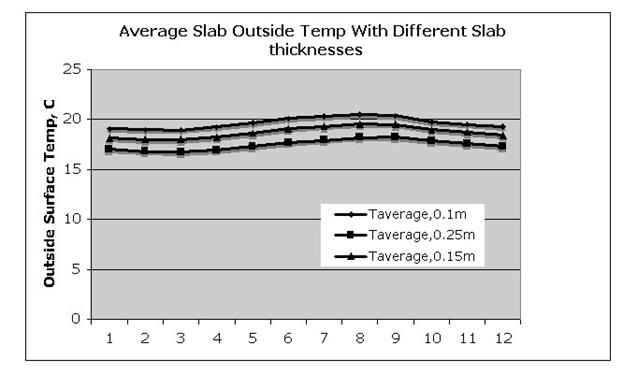
\includegraphics[width=0.9\textwidth, height=0.9\textheight, keepaspectratio=true]{media/image019.jpg}
\caption{Graph of Slab Outside Temperature vs Slab Thickness \protect \label{fig:graph-of-slab-outside-temperature-vs-slab}}
\end{figure}

\textbf{The EquivSlab object and the EquivAutoGrid Objects that follow have been replaced by the EquivalentSlab object above. They are included in the idd so that old idf files can still be read.}

\subsection{EquivSlab Object - Obsolete}\label{equivslab-object---obsolete}

This object provides the basic information for running a model that uses the area over perimeter ratio of the slab to determine the size of an equivalent rectangular slab.

\subsubsection{Field APRatio: The area to perimeter ratio for this slab}\label{field-apratio-the-area-to-perimeter-ratio-for-this-slab-1}

This field specifies the area over perimeter ratio of the slab in meters.

\subsubsection{Field: EquivSizing}\label{field-equivsizing}

This field value should be TRUE. This means that the program will determine the dimensions of the equivalent slab that satisfactorily models the A/P ratio.

The object is shown below.

\begin{lstlisting}
EquivSlab,
\memo Using an equivalent slab allows non-rectangular shapes to be modeled accurately
\memo The simulation default should be EquivSizing = True
        N1, \field APRatio: The area to perimeter ratio for this slab
            \units m
        A1; \field EquivSizing:
            \note Flag: Will the dimensions of an equivalent slab
            \note be calculated (TRUE) or will the dimensions be input directly? (FALSE)
            \note It is recommended that EnergyPlus users use TRUE.
\end{lstlisting}

\subsection{EquivAutoGrid Object - Obsolete}\label{equivautogrid-object---obsolete}

This object provides the information needed by the program to automatically generate the calculation grid when the slab is described as an equivalent slab. It is necessary for EnergyPlus users because equivalent slab is the appropriate option.

\subsubsection{Field SLABDEPTH: Thickness of slab on grade}\label{field-slabdepth-thickness-of-slab-on-grade-1}

This field specifies the thickness of the slab in meters. Note that the slab top surface is level with the ground surface, so this is the depth into the ground. The slab depth has a significant effect on the temperature calculation, and it is also important for the auto-grid process. The finite difference grids are set in such a way that they use the slab thickness to determine the vertical grid spacing. Because of this, autogridding will fail if the slab thickness is specified larger than 0.25 meters. The program also is set up so that the slab is a single finite difference cell in the vertical direction. Thus, if the slab thickness is set too large, the accuracy of the calculation may be suspect. The results with three different slab thicknesses are shown below.

All other inputs for the runs were the same. It is clear that the slab thickness has a significant effect because of the horizontal component of conduction in both directions in the slab.

\subsubsection{Field CLEARANCE: Distance from edge of slab to domain edge}\label{field-clearance-distance-from-edge-of-slab-to-domain-edge-1}

This field specifies the distance from the slab to the edge of the area that will be modeled with the grid system. It is the basic size dimension that is used to set both the horizontal and vertical extent of the domain. The units are meters, and 15 meters is a reasonable value.

The EquivAutoGrid object is shown below.

\begin{lstlisting}
EquivAutoGrid, \memo  EquivAutoGrid only necessary when EquivSizing is true
               \memo  EnergyPlus users normally use this option.
        N1, \field SLABDEPTH: Thickness of slab on grade
            \note typical value = 0.1
            \units m
        N2; \field CLEARANCE: Distance from edge of slab to domain edge
            \note typical value = 15.0
            \units m
\end{lstlisting}

\subsection{Additional Objects}\label{additional-objects-000}

There are five additional objects in the IDD that can be used under very special situations by researchers who want to generate special calculation grids. They are normally not useful to EnergyPlus users. They will be shown as IDD sections only. They do not need to be in the IDF.

\begin{lstlisting}
AutoGrid,   \memo AutoGrid only necessary when EquivSizing is false
            \memo  Not normally needed by EnergyPlus users.
        N1, \field SLABX: X dimension of the building slab
            \note typical values = 0-60.0
            \units m
        N2, \field SLABY: Y dimension of the building slab
            \note typical values = 0-60.0
            \units m
        N3, \field SLABDEPTH: Thickness of slab on grade
            \note typical value = .1
            \units m
        N4; \field CLEARANCE: Distance from edge of slab to domain edge
            \note typical value = 15.0
            \units m
\end{lstlisting}

\begin{lstlisting}
ManualGrid, \memo Manual Grid only necessary using manual gridding (not recommended)
            \memo   Used only in special cases.
        N1, \field NX: Number of cells in the X direction
            \note typical values = 15
        N2, \field NY: Number of cells in the Y direction
            \note typical values = 15
        N3, \field NZ: Number of cells in the Z direction
            \note typical values = 15
        N4, \field IBOX: X direction cell indicator of slab edge
            \note typical values = 1-10
        N5; \field JBOX: Y direction cell indicator of slab edge
            \note typical values = 1-10
\end{lstlisting}

\begin{lstlisting}
XFACE,  \memo This is only needed when using manual gridding (not recommended)
        \memo XFACE: X Direction cell face coordinates: m
  N1, N2, N3, N4, N5, N6, N7, N8, N9, N10, N11, N12, N13, N14,
  N15, N16, N17, N18, N19, N20, N21, N22, N23, N24, N25, N26, N27, N28, N29,
  N30, N31, N32, N33, N34, N35, N36, N37, N38, N39, N40;
\end{lstlisting}

\begin{lstlisting}
YFACE,  \memo This is only needed when using manual gridding (not recommended)
        \memo YFACE: Y Direction cell face coordinates: m,
  N1, N2, N3, N4, N5, N6, N7, N8, N9, N10, N11, N12, N13, N14,
  N15, N16, N17, N18, N19, N20, N21, N22, N23, N24, N25, N26, N27, N28, N29,
  N30, N31, N32, N33, N34, N35, N36, N37, N38, N39, N40;
\end{lstlisting}

\begin{lstlisting}
ZFACE,  \memo This is only needed when usuing manual gridding (not recommended)
        \memo ZFACE: Z Direction cell face coordinates: m
        N1, N2, N3, N4, N5, N6, N7, N8, N9, N10, N11, N12, N13, N14,
        N15, N16, N17, N18, N19, N20, N21, N22, N23, N24, N25;
\end{lstlisting}

\subsection{Sample IDF File - Slab Program}\label{sample-idf-file---slab-program}

A sample IDF file is shown below.

\begin{lstlisting}

!-Generator IDFEditor 1.12
  !-NOTE: All comments with '!-' are ignored by the IDFEditor and are generated automatically.
  !-      Use '!' comments if they need to be retained when using the IDFEditor.

  !-   = = = = = = = = = = =  ALL OBJECTS IN CLASS: MATERIALS = = = = = = = = = = =

  Materials,
  2,           !- NMAT: Number of materials
  0.158,       !- ALBEDO: Surface Albedo: No Snow
  0.379,       !- ALBEDO: Surface Albedo: Snow
  0.9,         !- EPSLW: Surface Emissivity: No Snow
  0.9,         !- EPSLW: Surface Emissivity: Snow
  0.75,        !- Z0: Surface Roughness: No Snow
  0.03,        !- Z0: Surface Roughness: Snow
  6.13,        !- HIN: Indoor HConv: Downward Flow {W/m2-K}
  9.26;        !- HIN: Indoor HConv: Upward {W/m2-K}

  !-   = = = = = = = = = = =  ALL OBJECTS IN CLASS: MATLPROPS = = = = = = = = = = =

  MatlProps,
  2300,        !- RHO: Slab Material density {kg/m3}
  1200,        !- RHO: Soil Density {kg/m3}
  653,         !- CP: Slab CP {J/kg-K}
  1200,        !- CP: Soil CP {J/kg-K}
  0.93,        !- TCON: Slab k {W/m-K}
  1;           !- TCON: Soil k {W/m-K}

  !-   = = = = = = = = = = =  ALL OBJECTS IN CLASS: BOUNDCONDS = = = = = = = = = = =

  BoundConds,
  TRUE,        !- EVTR: Is surface evapotranspiration modeled
  TRUE,        !- FIXBC: is the lower boundary at a fixed temperature
  FALSE;       !- OLDTG: is there an old ground temperature file

  !-   = = = = = = = = = = =  ALL OBJECTS IN CLASS: BLDGPROPS = = = = = = = = = = =

  BldgProps,
  10,          !- IYRS: Number of years to iterate
  0,           !- Shape: Slab shape
  4,           !- HBLDG: Building height {m}
  18,          !- TIN1: January Indoor Average temperature set point {C}
  18,          !- TIN2: February Indoor Average temperature set point {C}
  18,          !- TIN3: March Indoor Average temperature set point {C}
  20,          !- TIN4: April Indoor Average temperature set point {C}
  20,          !- TIN5: May Indoor Average temperature set point {C}
  20,          !- TIN6: June Indoor Average temperature set point {C}
  22,          !- TIN7: July Indoor Average temperature set point {C}
  22,          !- TIN8: August Indoor Average temperature set point {C}
  22,          !- TIN9: September Indoor Average temperature set point {C}
  22,          !- TIN10: October Indoor Average temperature set point {C}
  20,          !- TIN11: NovemberIndoor Average temperature set point {C}
  20,          !- TIN12: December Indoor Average temperature set point {C}
  0,           !- TINAmp: Daily sine wave variation amplitude {C}
  0.10;        !- ConvTol: Convergence Tolerance

  !-   = = = = = = = = = = =  ALL OBJECTS IN CLASS: INSULATION = = = = = = = = = = =

  Insulation,
  0.,          !- RINS: R value of under slab insulation {m2-K/W}
  0.,          !- DINS: Width of strip of under slab insulation {m}
  2.0,         !- RVINS: R value of vertical insulation {m2-K/W}
  2.0,         !- ZVINS: Depth of vertical insulation {m}
  1;           !- IVINS: Flag: Is there vertical insulation

  !-   = = = = = = = = = = =  ALL OBJECTS IN CLASS: EQUIVSLAB = = = = = = = = = = =

  EquivalentSlab,
  10,          !- APRatio: The area to perimeter ratio for this slab {m}
  0.1,         !- SLABDEPTH: Thickness of slab on grade {m}
  15,          !- CLEARANCE: Distance from edge of slab to domain edge {m}
  10;          !-ZCLEARANCE: Distance from bottom of slab to domain bottom
\end{lstlisting}
